\documentclass[border=10pt]{standalone}

\usepackage{tikz}
\usepackage{tikzsymbols}
\usetikzlibrary{calc,patterns,shapes.geometric}

\def\centerarc[#1](#2)(#3:#4:#5){\draw[#1] ($(#2)+({#5*cos(#3)},{#5*sin(#3)})$) arc (#3:#4:#5);}

\begin{document}
	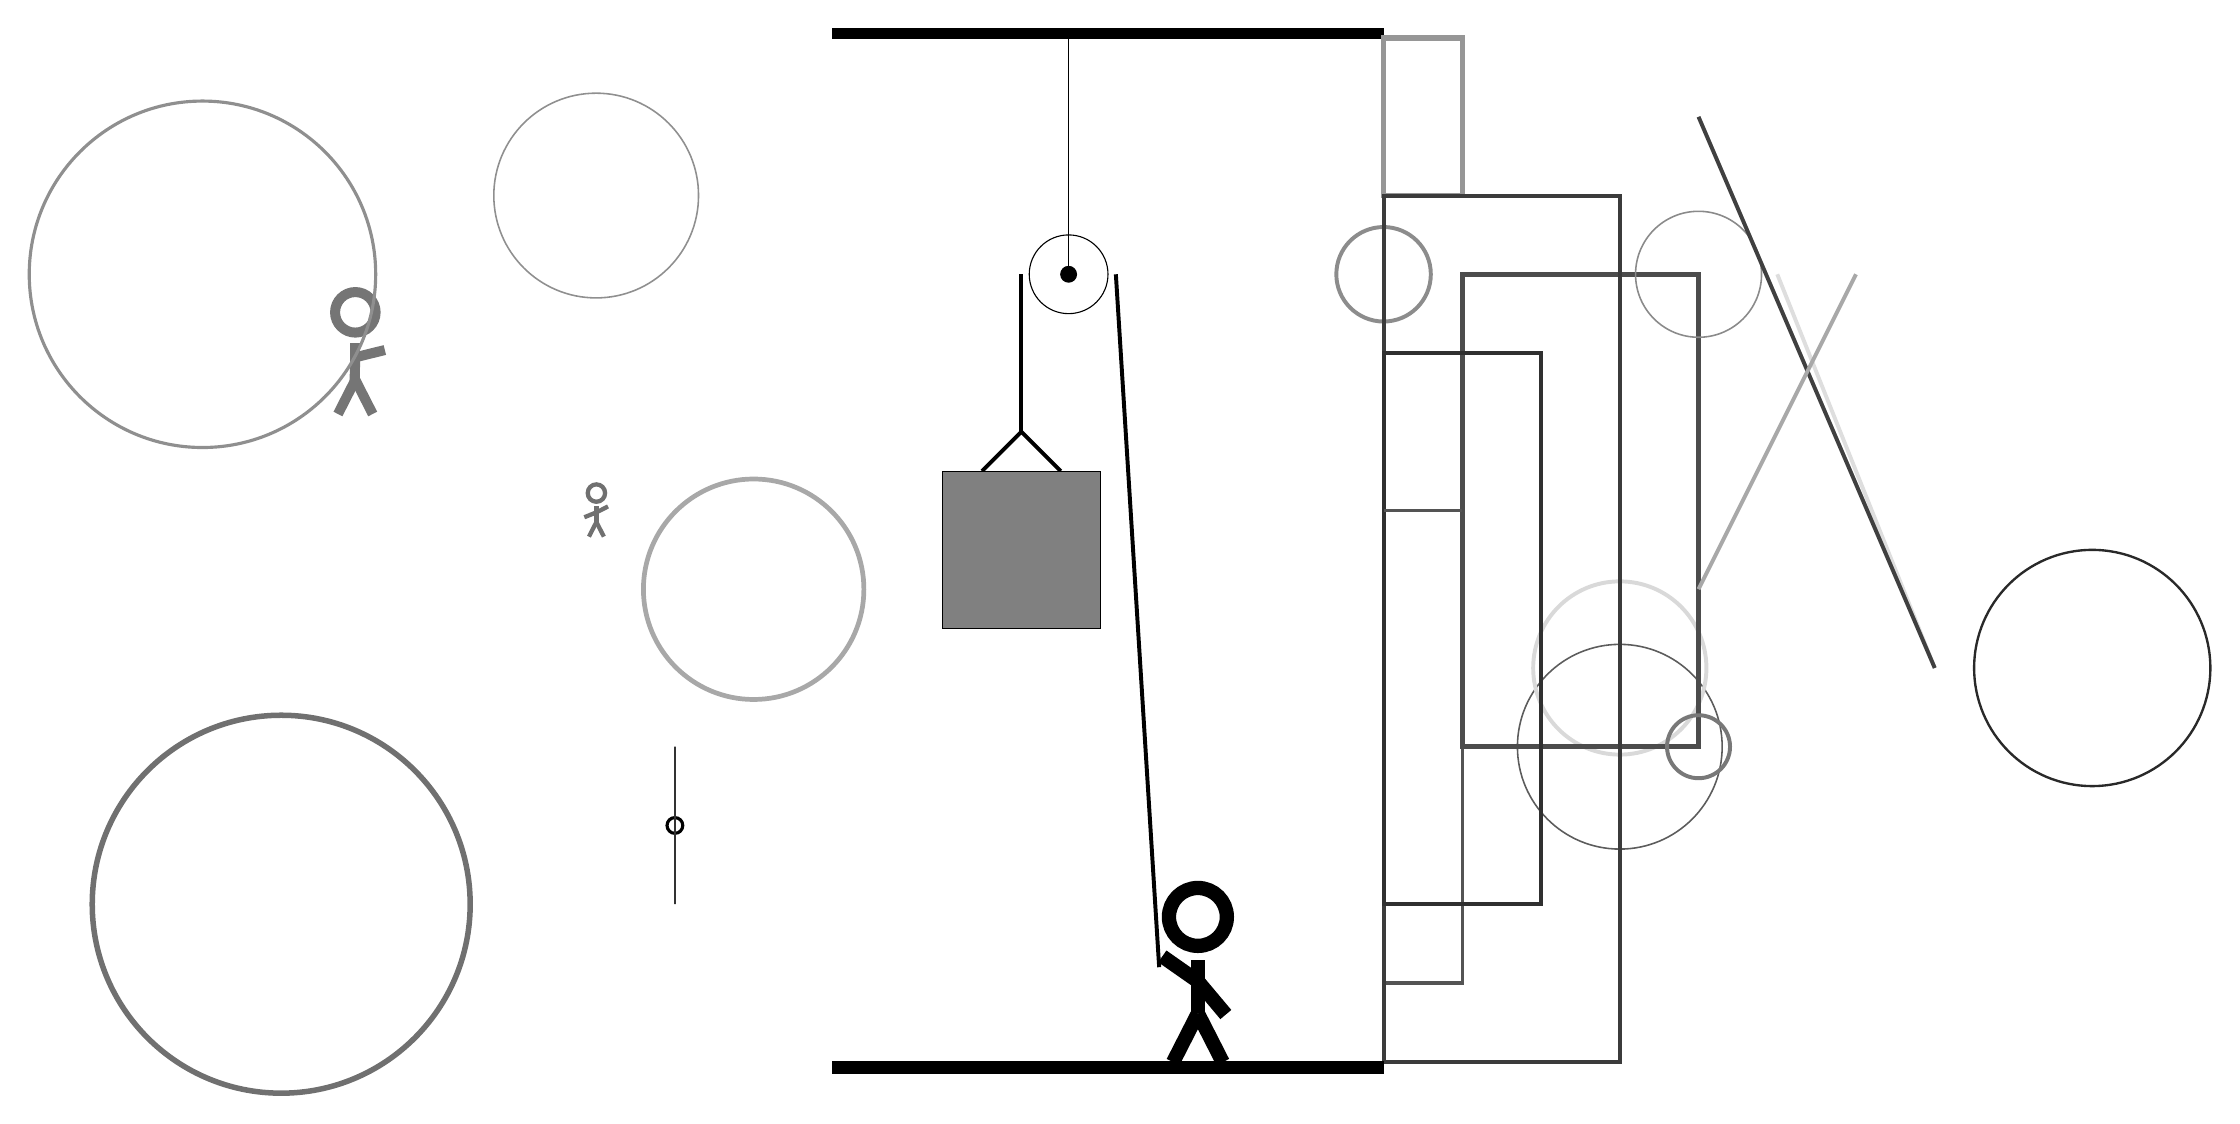
\begin{tikzpicture}
		%%%%% START %%%%%
		
		\draw[fill=black] (-2, 10) rectangle (5, 10.125);
		
		\draw (1, 7) circle (0.5);
		\draw[fill=black] (1, 7) circle (0.1);
		\draw (1, 10) -- (1, 7);
		
		\draw[line width=0.5mm] (-0.1, 4.5) -- (0.4, 5.0) -- (0.9, 4.5);
		\draw[fill=black!50] (-0.6, 4.5) rectangle (1.4, 2.5);
		
		\draw[line width=0.5mm] (0.4, 7) -- (0.4, 5.0);
		\centerarc[line width=0.5mm](1, 7)(0:180:0.6);
		\draw[line width=0.5mm](1.6, 7) -- (2.15, -1.8);
		
		\draw [line width=0.2mm, color=black!64](8, 1) circle (1.3);
		
		\node[line width=0.2mm, color=black!54] at (-8, 6) {\Strichmaxerl[7][88][14]};
		\node[line width=0.5mm, color=black!56] at (-5, 4) {\Strichmaxerl[3][22][27]};
		\draw [line width=0.2mm, color=black!44](-5, 8) circle (1.3);
		
		\draw[line width=0.4mm, color=black!67] (5, 4) rectangle (6, -2);
		
		\draw [line width=0.5mm, color=black!15](8, 2) circle (1.1);
		\draw[line width=0.7mm, color=black!41] (5, 8) rectangle (6, 10);
		\draw [line width=0.3mm, color=black!84](14, 2) circle (1.5);
		\draw[line width=0.7mm, color=black!70] (6, 1) rectangle (9, 7);
		\draw [line width=0.4mm, color=black!100](-4, 0) circle (0.1);
		\draw[line width=0.5mm, color=black!13](10, 7) -- (12, 2);
		
		\draw [line width=0.6mm, color=black!34](-3, 3) circle (1.4);
		\draw [line width=0.2mm, color=black!46](9, 7) circle (0.8);
		
		\draw [line width=0.5mm, color=black!53](9, 1) circle (0.4);
		\draw[line width=0.5mm, color=black!75](9, 9) -- (12, 2);
		\draw [line width=0.5mm, color=black!45](5, 7) circle (0.6);
		\draw[line width=0.5mm, color=black!34](9, 3) -- (11, 7);
		\draw [line width=0.4mm, color=black!44](-10, 7) circle (2.2);
		\draw[line width=0.5mm, color=black!77] (5, 8) rectangle (8, -3);
		\draw[line width=0.5mm, color=black!81] (7, 6) rectangle (5, -1);
		\draw [line width=0.7mm, color=black!56](-9, -1) circle (2.4);
		
		\draw[line width=0.2mm, color=black!80] (-4, 1) rectangle (-4, -1);
		\draw[line width=0.5mm, color=black!67](5, 4) -- (6, 4);
		
		\node at (2.6, -1.9) {\Strichmaxerl[10][-35][-50]};
		
		\draw[fill=black] (-2, -3) rectangle (5, -3.15);
		
		%%%%% END %%%%%
	\end{tikzpicture}
\end{document}